\section{Lexikalische Analyse}
\subsection{Lexer / Scanner}
\textbf{Endlicher Automat (DEA)}
\begin{itemize}
    \item Kümmert sich um die lexikalische Analyse
    \item Input: Zeichenfolge (Programmtext)
    \item Output: Folge von Terminalsymbolen (Tokens)
\end{itemize}
\subsubsection{Aufgaben}
\begin{itemize}
    \item Fasst Textzeichen zu tokens zusammen
    \item Eliminiert Whitespaces
    \item Eliminiert Kommentare
    \item Merkt Positionen in Programmcode
\end{itemize}
\subsubsection{Nutzen}
\textbf{Abstraktion}
\begin{itemize}
    \item Parser muss sich nicht um Textzeichen kümmern
\end{itemize}
\textbf{Einfachheit}
\begin{itemize}
    \item Parser braucht Lookahead pro Symbol, nicht Textzeichen
\end{itemize}
\textbf{Effizienz}
\begin{itemize}
    \item Lexer benötigt keinen Stack im Gegensatz zu Parser
\end{itemize}

\subsection{Tokens}
\textbf{Statisch (Keywords, Operationen, Interpunktion)}
\begin{itemize}
    \item \textit{if}
    \item \textit{else}
    \item \textit{while}
    \item \textit{*}
    \item \textit{\&\&}
    \item \textit{;}
\end{itemize}
\textbf{Identifiers}
\begin{itemize}
    \item MyClass
    \item readFile
    \item name2
\end{itemize}
\textbf{Zahlen}
\begin{itemize}
    \item 123
    \item 0xfe12
    \item 1.2e-3
\end{itemize}
\textbf{Strings}
\begin{itemize}
    \item \dq Hello\dq
    \item \dq \dq
    \item \dq $\backslash$n\dq
\end{itemize}
\begin{center}
    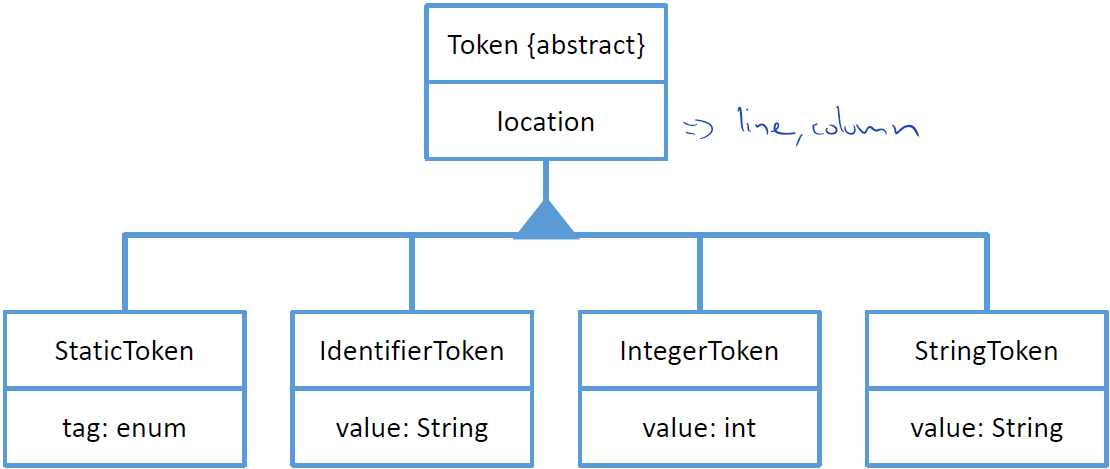
\includegraphics[width=0.4\linewidth]{/token_model.png} 
\end{center}

\subsubsection{Lexem}
\begin{itemize}
    \item Spezifische Zeichenfolge, die einen Token darstellt
    \item z.B. \textit{MyClass} ist ein Lexem des Tokens Identifier
\end{itemize}

\subsubsection{Maximum Munch}
\begin{itemize}
    \item Lexer absorbiert möglichst viel in einem Token
\end{itemize}

\subsection{Reguläre Sprachen}
\begin{itemize}
    \item Lexer unterstützt nur reguläre Sprachen
    \item \textbf{Regulär:} Als EBNF ohne Rekursion ausdrückbar
\end{itemize}
\begin{center}
    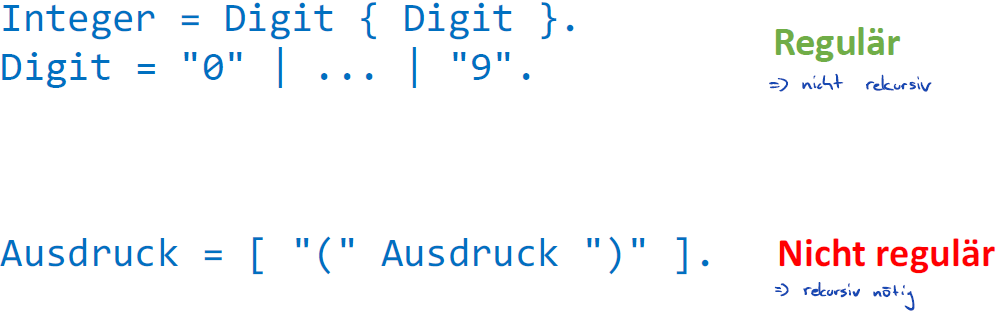
\includegraphics[width=0.5\linewidth]{/reg_sprachen.png} 
\end{center}

\subsection{Chomsky Hierarchie}
\begin{center}
    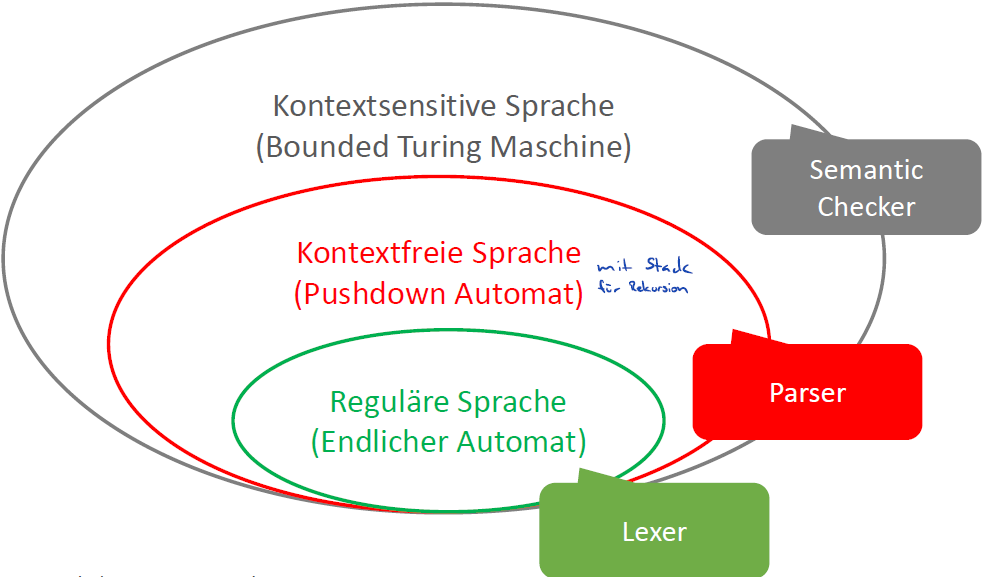
\includegraphics[width=0.7\linewidth]{/chomsky.png} 
\end{center}

\subsection{Lexer Gerüst}
\begin{lstlisting}
class Lexer {
    private final Reader reader;
    private char current; // one Character Lookahead
    private boolean end; // EOF 

    private Lexer(Reader reader) {
        this.reader = reader;
    }

    public static Iterable<Token> scan(Reader reader) {
        return new Lexer(reader).readTokenStream();
    }

    // ...
}
\end{lstlisting}

\subsection{Token Stream lesen}
\begin{lstlisting}
Iterable<Token> readTokenStream() {
    var stream = new ArrayList<Token>();
    readNext(); // One Character Lookahead
    skipBlanks();
    while (!end) {
        stream.add(readToken());
        skipBlanks();
    }
    return stream;
}
\end{lstlisting}

\subsection{Lexer Kernlogik}
\begin{lstlisting}
Token readToken() {
    if(isDigit(current)) {
        return readInteger();
    }
    if(isLetter(current)) {
        return readName(); // Identifier / Keyword 
    }
    return switch(current) {
        case '"': readString();
        case '+': readStaticToken(Tag.Plus);
        case '-': readStaticToken(Tag.Minus);
        case '/': readPotentialSlash();
    }
}
\end{lstlisting}

\subsubsection{Static Token scannen}
\begin{lstlisting}
StaticToken readStaticToken(Tag tag) {
    readNext();
    return new StaticToken(tag);
}
\end{lstlisting}

\subsubsection{Zahlen scennen}
\textbf{Beachten:}
\begin{itemize}
    \item Range Check (32 bit): Integer Overflow
    \item $Integer.MIN$ = $Integer.MAX+1$
\end{itemize}
\begin{lstlisting}
IntegerToken readInteger() {
    int value = 0;
    while (!_end && isDigit(current)) {
        int digit = current - '0'; // char to int 
        value = value * 10 + digit; // create decimal number
        readNext();
    }
    return new IntegerToken(value);
}
\end{lstlisting}

\subsubsection{Identifier und Keywords scannen}
\begin{lstlisting}
Token readName() {
    String name = Character.toString(current);
    readNext();
    while(!end & (isLetter(current) || isDigit(current))) {
        name += current;
        readNext();
    }
    if(KEYWORDS.containsKey(name)) {
        return new StaticToken(KEYWORDS.get(name));
    }
    return new IdentifierToken(name);
}
\end{lstlisting}

\subsubsection{String scannen}
\textbf{Beachten:}
\begin{itemize}
    \item Kein $\backslash$t
    \item Kein $\backslash$\dq
    \item Kein $\backslash$n
    \item Keine mehrzeiligen Strings
\end{itemize}
\begin{lstlisting}
StringToken readString() {
    readNext(); // Skip leading double Quote
    String value = "";
    while (!end && current != '"') {
        value += current;
        readNext();
    }
    if(end) {
        // Error: String not closed
    }
    readNext(); // Skip trailing double Quote
    return new StringToken(value);
}
\end{lstlisting}

\subsubsection{Kommentare erkennen}
\begin{lstlisting}
StaticToken readPotentialSlash() {
    readNext();
    if(current == '/') {
        skipLineComment();
        // move on to next token
    } else if (current == '*') {
        skipCommentBlock();
        // move on to next token
    } else {
        return new StaticToken(Tag.Divide);
    }
}
\end{lstlisting}